
\paragraph{Motivation}

Unmanned Aircraft System (UAS) are expected to proliferate in low-altitude airspace over the coming decade. Drones with vertical takeoff and landing (VTOL) capability have been proposed to offer fast package delivery, monitor and secure assets, perform inspections, and entertain.
% The \acf{FAA} estimates over 1.25 million \acf{sUAS} were flown in 2018 \cite{federal_aviation_administration_unmanned_2019}, far exceeding the number of registered manned aircraft in the USA.  Many \ac{sUAS} are  configured for \acf{VTOL} because of requirements for minimal area for ingress and egress in cities.  
Low-altitude operation of UAS in urban areas will require flight near buildings and over people. 
% Safety must be a top priority for system designers and regulators as UAS will pose new risks to the overflown population.
A primary safety concern is ensuring a robust urgent landing capability \cite{winnefeld_unmanned_2011,degarmo_issues_2013}.  Urgent landing requires landing site selection, trajectory planning, and stable flight control to actually reach the selected site \cite{atkins_emergency_2006}. It is possible a UAS may identify a safe site within sensor range allowing for an immediate landing.  However, when no safe site is within range the UAS must devote time and energy to exploring sites beyond sensor range or else utilize pre-processed data to identify a safe site \cite{ten_harmsel_emergency_2017,ochoa_fail-safe_2017}.  An onboard database of maps including landing sites can be incorporated into an efficient autonomous decision making framework \cite{sankararaman_towards_2017}. Offline data sources such as satellite images, airborne LiDAR point clouds, and existing map data may be used to aid map construction.
% Such a framework should incorporate risk models which account for both the intrinsic risk of the landing site as well as the path risk to reach the landing site.
% For example, Refs.  \cite{atkins_emergency_2006, meuleau_emergency_2009}  and \cite{sankararaman_towards_2017} utilize airborne flight risk models to build emergency landing plans for fixed-wing and urban flight operations, respectively. We call such a decision making framework a map-based planner.

Conventional fixed-wing emergency landing sites such as open fields and roadways are either extremely rare or highly populated in and around cities. Consider the satellite image in Figure \ref{fig:ch1_challenge_urban} which shows the typical sparsity of conventional landing zones in the city Witten, Germany. However, these images show a multitude of unoccupied flat rooftops that may provide nearby landing sites for small lightweight UAS. Obstacles such as air conditioning units, skylights, and rooftop entrances on these surfaces may be present and must be explicitly modeled and avoided during an urgent landing. Polygons can accurately and simply represent these flat surfaces as well as obstacles embedded on them per Figure \ref{fig:ch1_roof_shape_obstacle}. Archived data can be processed such that rooftop landing sites substantially augment existing conventional landing site databases.






% \acf{GIS} use polygons in vector map data to represent many items such as parks, fields, and buildings outlines. 
% This dissertation will have a strong focus on creating databases of such flat surfaces using efficient computational geometry routines coupled with deep learning.  


% \begin{figure}[ht]
%     \centering
%     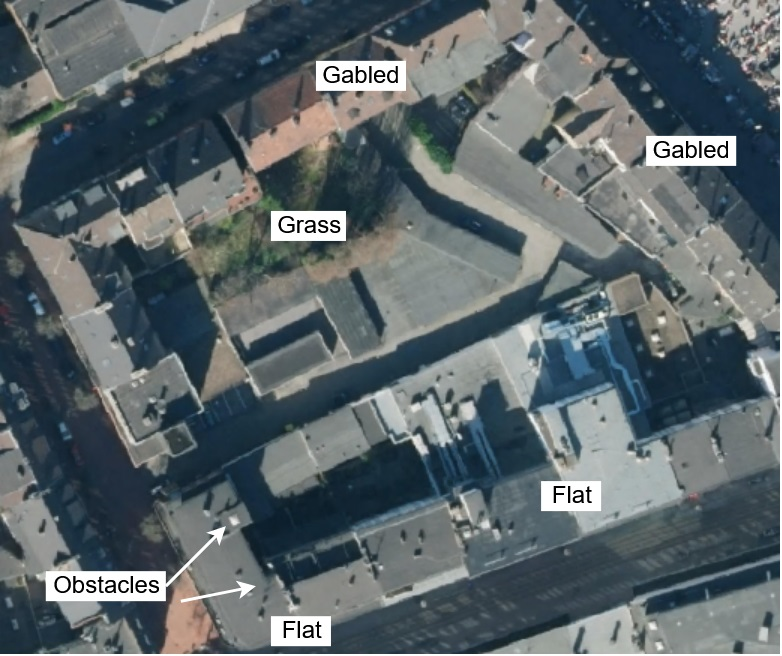
\includegraphics[clip, trim=0.0cm 0cm 0cm 0cm, width=0.55\linewidth]{chapter_5_mapping/imgs/challenge_urban-Page-2.jpg}
%     \caption{Satellite image of an urban environment with multiple flat roof landing sites. Select roof shapes and obstacles are labeled.}
%     \label{fig:ch1_challenge_urban}
% \end{figure}


\begin{figure}[ht]
    \centering
  \begin{subfigure}{.45\linewidth}
    \centering
    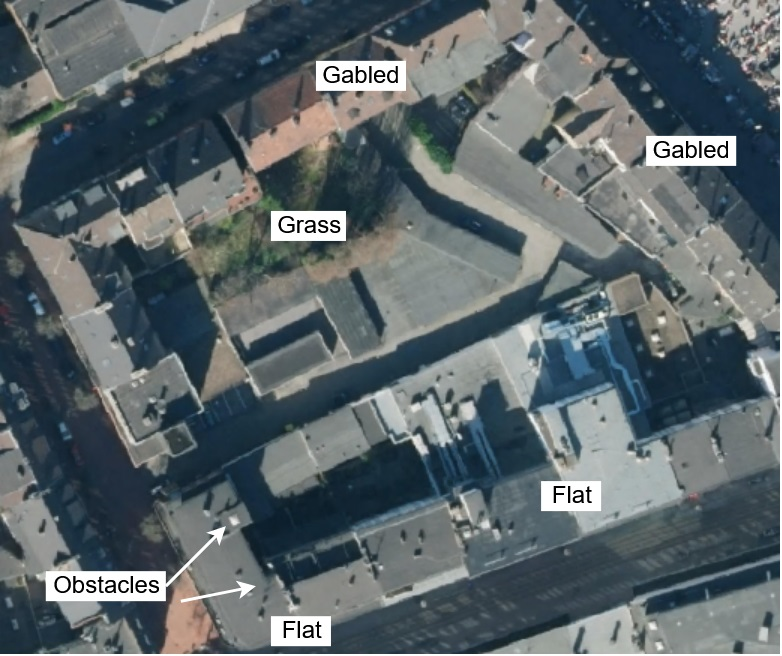
\includegraphics[clip, trim=0.0cm 0cm 0cm 0.55cm, width=0.95\linewidth]{chapter_5_mapping/imgs/challenge_urban-Page-2.jpg}
    \caption{}
    \label{fig:ch1_challenge_urban}
  \end{subfigure}
  \begin{subfigure}{.45\linewidth}
    \centering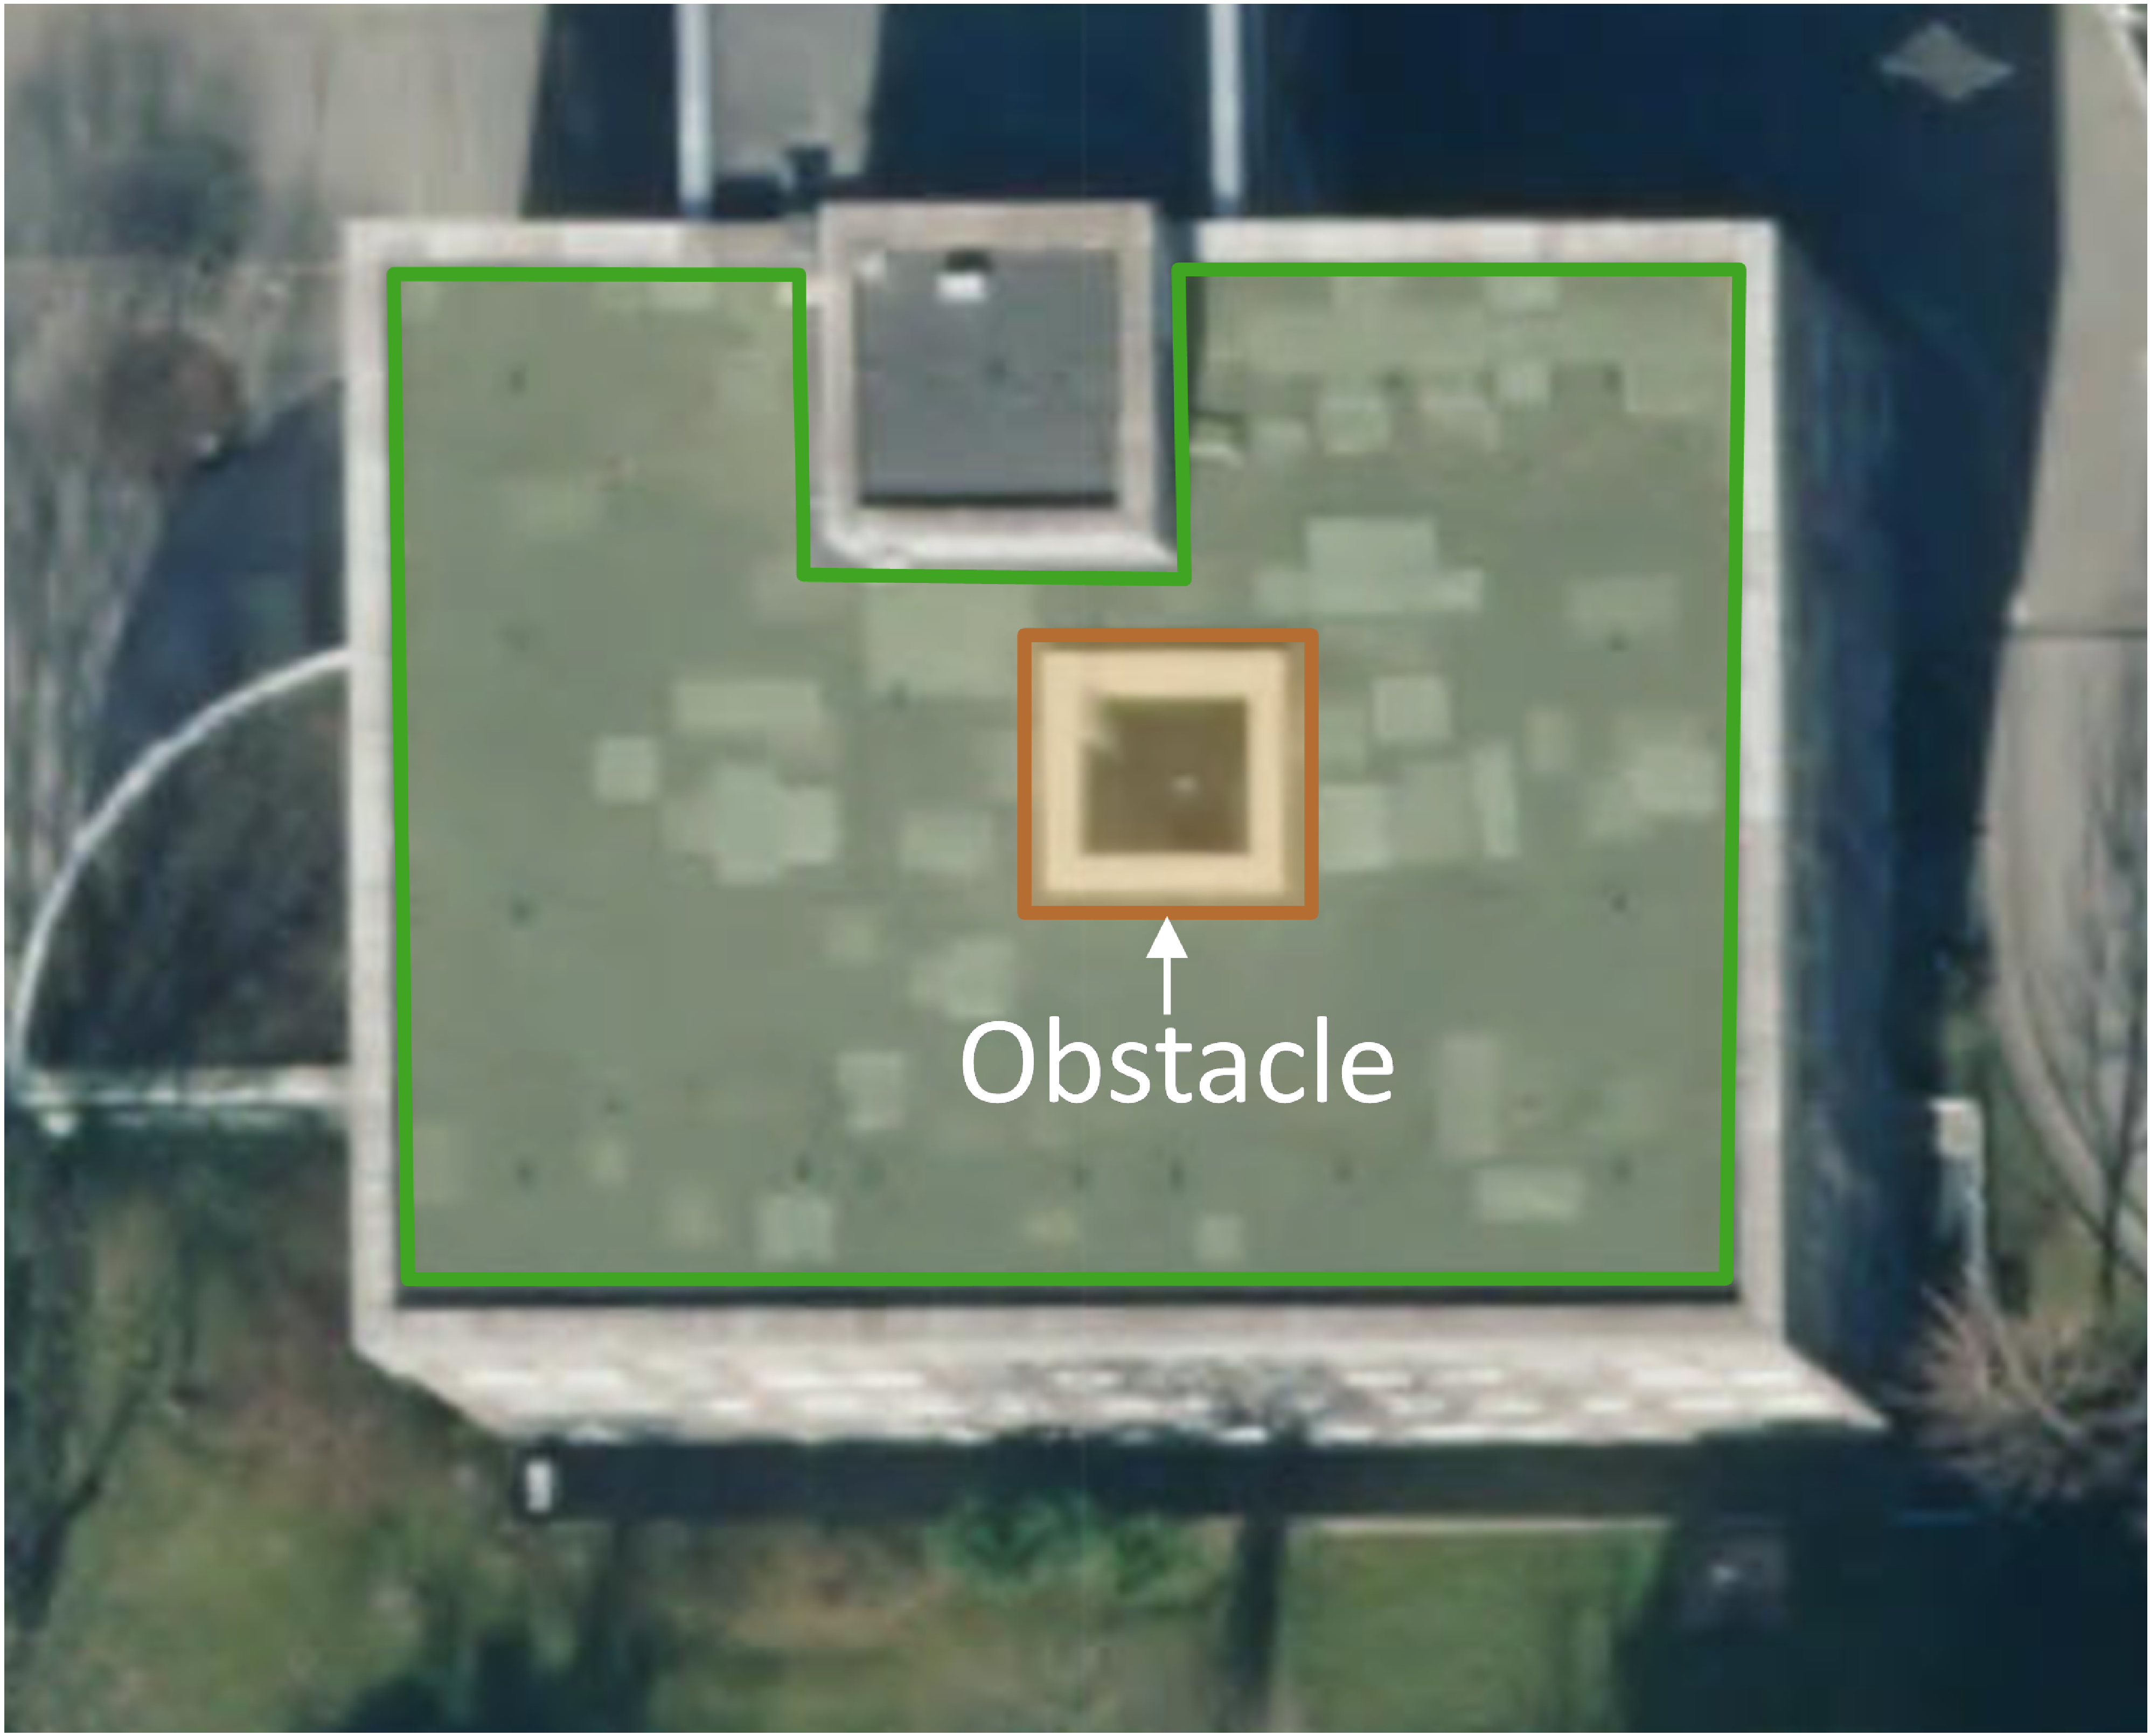
\includegraphics[width=.95\linewidth]{chapter_1_intro/imgs/roof_shape_obstacle.pdf}
    \caption{}
    \label{fig:ch1_roof_shape_obstacle}
  \end{subfigure}
  \caption{(\subref{fig:ch1_challenge_urban}) Satellite image of an urban environment with multiple flat rooftops. Select roof shapes and obstacles are labeled.  (\subref{fig:ch1_roof_shape_obstacle}) A rooftop surface can be represented as a non-convex polygon with an exterior shell (green) and interior hole(s) (orange).  }\label{fig:ch1_motivation}
\end{figure}




\paragraph{Problem Statement}

This dissertation aims to address the following challenges:

\begin{enumerate}[noitemsep]
    \itemsep0em 
    \item Where can a small UAS safely land in a city during an urgent or emergency landing situation?
    \item How can maps be constructed and risk evaluated for landing site selection and path planning?
    % \item What path should it take reach this landing site?
    \item How can the small UAS verify a landing zone is safe in real-time on approach to that site?
\end{enumerate}

Previous research has proposed the use of public Geographic Information Systems (GIS) datasets such as satellite images, airborne LiDAR point clouds, digital elevation maps, census data, and building outlines for terrain-based landing site identification, risk assessment, and path planning \cite{meuleau_emergency_2009, di_donato_evaluating_2017, patterson_timely_2014, bleier_risk_2015}.  However increased use of sUAS in urban cities motivates this work to additionally consider building rooftops as landing sites. To our knowledge this dissertation is the first work to explicitly use GIS data to automatically identify flat rooftop buildings, isolate flat surfaces, and find risk-minimum touchdown points that maximize distance to obstacles. 

% These conventional landing sites are often risk evaluated by terrain type and size \cite{di_donato_evaluating_2017}. 
\paragraph{Research Approach}

% Map data is widely available in vector form, such as polygons, which describes features such as fields, parks, and building outlines \cite{openstreetmap_contributors_planet_2017}.  Such polygons can be efficiently stored and indexed such that spatial queries may efficiently computed in an embedded database \cite{furieri_spatialite_2017}. 

This dissertation proposes to process existing GIS data to extract safe landing sites and occupancy maps used for map-based planning. To accomplishing this several computational geometry algorithms have been developed to enable efficient extraction of flat surfaces as non-convex polygons. The overall structure of this dissertation is shown in Figure \ref{fig:ch1_thesis_overview} and can be summarized as accomplishing the following six tasks:
% This dissertation assumes these urgent landing scenarios are without loss-of-control, for example: low battery energy, lost communication link, adverse weather, non-essential sensor or actuator failure, operator emergency landing directive, and non-cooperative aircraft nearby.

\begin{enumerate}[noitemsep]
    \item Efficiently extract non-convex polygons with interior holes from 2D point sets. (Ch. 2)
    \item Extend polygon extraction methods from 2D point sets to 3D data where polygons represent flat surfaces and interior holes represent obstacles embedded on the surface. (Ch. 3)
    \item Classify rooftop shape in a city (e.g., flat) with high confidence in model prediction. (Ch. 4)
    \item Assimilate publicly available GIS data such as satellite images, airborne LiDAR point clouds, and existing map data into an urgent landing site database with associated risk metrics as well as occupancy maps for path planning. (Ch. 5)
    \item Create a multi-goal planner to efficiently search through candidate sites and account for landing site risk as well as flight path risk to that site. The planner identifies a landing site/path pair to minimize combined \emph{total} risk as well as computation time for this search. (Ch. 5)
    \item Perform experiments to verify the planned touchdown location is safe in real-time using on-board sensors such as LiDAR. (Ch. 6, Proposed)
\end{enumerate}

% The final risk-optimal landing site/path pair is sent to a navigation controller.
\begin{figure}[t]
    \centering
    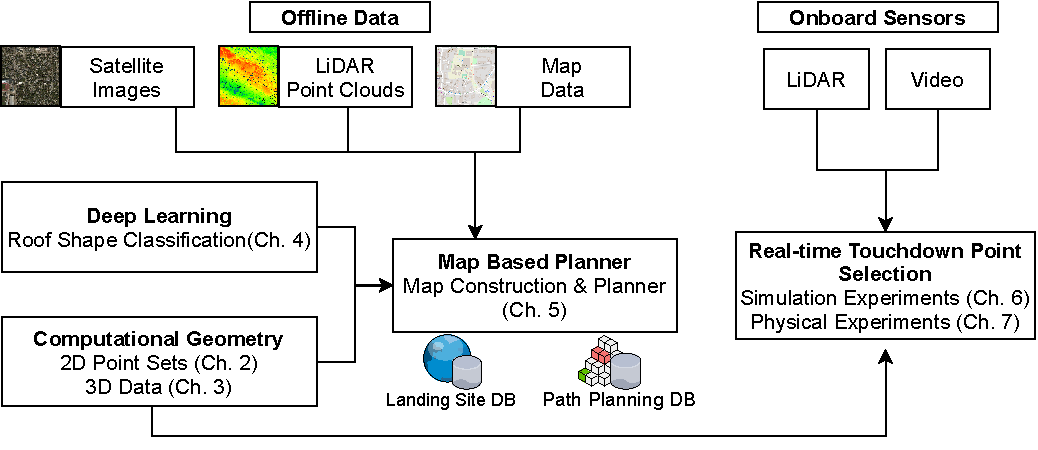
\includegraphics[width=0.70\linewidth]{chapter_1_intro/imgs/Challenge_Overview-thesis_overview.pdf}
    \caption{Overview of dissertation topics and structure.}
    \label{fig:ch1_thesis_overview}
\end{figure}

% \emph{How to efficiently construct databases from publicly available data to identify minimal-risk landing site for sUAS.}. Our previous stated observation of flat rooftop motivates 

% Numerous public datasets exist to aid construction of maps for aircraft urgent landing including satellite images, airborne LiDAR point clouds, census data, and existing building outlines. Our first goal is to efficiently transform this raw data into a risk evaluated landing site database which may be used for landing site selection and path planning.  Previous research has used such data to identity terrain based landing but none to our knowledge has focused on extracting flat rooftops \cite{atkins_emergency_2006, meuleau_emergency_2009, sankararaman_towards_2017, di_donato_evaluating_2017}. Our second goal is the construction of an efficient multi-goal planner which will account for both the intrinsic landing site risk as well as path risk. 



% Talk about data. Talk about the forms of data we have available for us to use: satellite images, airborne lidar points clouds, building outlines, census data. A host of information to help us make decision about places we can land.


\paragraph{Polygons from 2D Point Sets}

Characterizing the shape of a set of 2D points $\mathcal{P}$ has been a long-term focus of computational geometry research. A convex hull is defined as the smallest convex polygon that fully encapsulates all points in a set $\mathcal{P}$ as shown in Figure \ref{fig:ch1_convex_concave_1}.  Although widely used to estimate shape, point sets with non-convex distributions are poorly characterized by a convex hull \cite{duckham_efficient_2008}.  Convex hull over-estimation can be a serious issue when the points represent physical objects, e.g., obstacle free navigable areas. Several algorithms have been developed to construct shapes that ``fit'' or ``cover'' point sets more closely. These shapes are often termed non-convex polygons or concave hulls. 

The most notable examples of these algorithms are $\alpha$-shape \cite{edelsbrunner_shape_1983}, Spatialite concave hull \cite{furieri_spatialite_2017}, and PostGIS concave hull \cite{open_source_geospatial_foundation_postgis_2019}. Each is widely used in the computational geometry and GIS communities. These methods can extract the exterior boundary of a point set and also interior holes.  However, many of these methods are extremely slow motivating this dissertation to create an efficient non-convex (multi)polygon extraction algorithm called Polylidar. A key insight of this work is a novel boundary following method that contrasts computationally-expensive geometric unions of triangles. Real-world and synthetic benchmarks are presented to comparatively evaluate Polylidar speed and accuracy. Results show comparable accuracy and more than four times speedup compared to other open source concave polygon extraction methods. An example polygon from Polylidar is shown in Figure \ref{fig:ch1_convex_concave_2}.

% This dissertation uses the Open GeoSpatial Consortium (OGC) standard \cite{herring_opengis_2006-1} for defining \textit{linear ring} and \textit{polygon}. A linear ring is a consecutive list of points that is both closed and simple. This requires a linear ring to have non-intersecting line segments that join to form a closed path. The key components of a valid polygon are a single exterior linear ring representing the \emph{shell} of the polygon and a set of linear rings (possibly empty) representing \emph{holes} inside the polygon. 


\begin{figure}[t]

  \begin{subfigure}[t]{.22\linewidth}
    \centering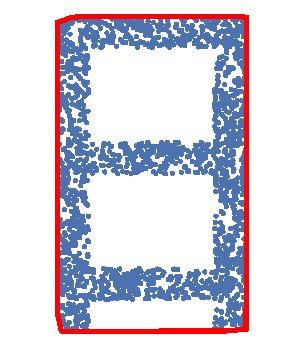
\includegraphics[width=.95\linewidth]{chapter_3_polylidar3d/imgs/concave_vs_convex_lettera_1.pdf}
    \caption{\label{fig:ch1_convex_concave_1}}
  \end{subfigure}
  \begin{subfigure}[t]{.22\linewidth}
    \centering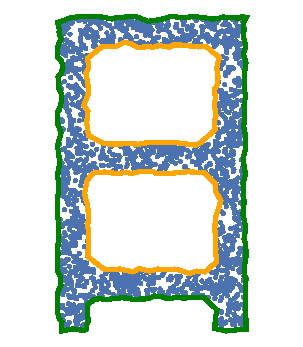
\includegraphics[width=.95\linewidth]{chapter_3_polylidar3d/imgs/concave_vs_convex_lettera_3.pdf}
    \caption{\label{fig:ch1_convex_concave_2}}
  \end{subfigure}
  \begin{subfigure}[t]{.26\linewidth}
    \centering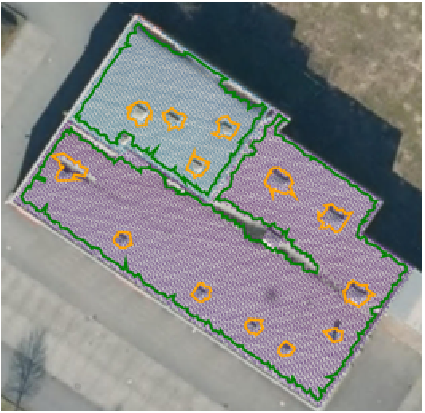
\includegraphics[width=.95\linewidth]{chapter_1_intro/imgs/rooftop_example_simple.pdf}
    \caption{\label{fig:ch1_rooftop_polygon}}
  \end{subfigure}
  \begin{subfigure}[t]{.26\linewidth}
    \centering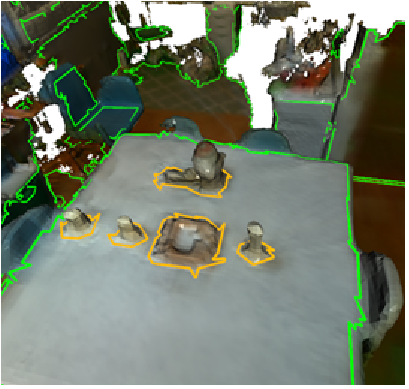
\includegraphics[width=.95\linewidth]{chapter_1_intro/imgs/mesh_example_simple.pdf}
    \caption{\label{fig:ch1_mesh_polygon}}
  \end{subfigure}
  \caption{(a,b) Examples of a convex hull (red) and a non-convex polygon with holes from a 2D point set. (c,d) Examples of Polylidar3D's non-convex multi-polygon extraction from airborne LiDAR point clouds (colored by height) and a user provided mesh, respectively}\label{fig:ch1_polygon_examples}
\end{figure}


\paragraph{Polygons from 3D Data}

Flat surfaces are pervasive in engineered structures and also occur in natural terrain. For example, structures such as walls, floors, rooftops, and roadways are often flat or ``flat-like". 
% Similarly, home and office furnishings are typically composed of multiple flat surfaces.
Sensors such as LiDAR and RGBD cameras generate dense 3D point clouds of these predominately flat surface environments. This observation has been exploited for tasks in localization and mapping \cite{pathak_online_2010},  digital preservation with Photogrammetry and laser scanning \cite{malihi_3d_2016, lerma_terrestrial_2010, balsa-barreiro_generation_2018}, and point cloud registration \cite{rusinkiewicz_efficient_2001}. Planar segmentation techniques are often used to group points belonging to a common flat surface \cite{feng_fast_2014, pham_geometrically_2016-1, schaefer_maximum_2019}. However points clouds are dense incurring high computational cost when used directly in higher level tasks. Planar point clouds can be converted to lower dimensional representations such as polygons.
% Polygons reduce map size, accelerate matching for localization \cite{lee_indoor_2012-1}, and support model reconstruction and object detection \cite{cao_roof_2017}. 

Prior work has investigated transforming planar points clouds to convex polygons \cite{biswas_planar_2012,poppinga_fast_2008}.  Non-convex polygons can be generated using techniques such as $\alpha$-shapes but operate strictly on 2D data, requiring the projection of each 3D planar point cloud and expensive triangulation \cite{lee_fast_2013, edelsbrunner_shape_1983}. Pixel-level boundary following of organized point clouds (e.g., range images) can be used to extract non-convex polygons but often only captures the exterior shell of the polygon \cite{lee_indoor_2012-1}. These methods do not capture interior holes in a polygon needed to capture obstacles on flat surfaces. 

% Finally, many of the proposed solutions are limited in their use of 3D data, only working on range images and unable to handle unorganized forms of 3D data.

This dissertation introduces Polylidar3D, a non-convex polygon extraction algorithm that takes as input either unorganized 3D point clouds (e.g., airborne LiDAR point clouds), organized point clouds (e.g., range images), or user-provided meshes. A core idea of this work is to transform all data inputs into a half-edge triangular mesh for which planar segmentation and polygon extraction may occur in parallel. Dominant plane normals are identified and used to parallelize and regularize planar segments in the mesh. Triangles having similar normals to a dominant plane are grouped. Each group (in parallel) then performs region growing accounting for normal orientation, Euclidean distance, and point to plane distance. Immediately after a plane has been segmented a polygon extraction task is dynamically spawned. The result is a general and extremely fast framework for non-convex polygon extraction of 3D data. Polylidar3D is used in this dissertation to extract polygonal representations of flat rooftop surfaces and generated meshes as shown in Figure \ref{fig:ch1_polygon_examples}c,d.


% Speed is an important consideration for many of the applications mentioned previously. Parallel algorithms written for multi-core CPUs and GPUs should be used to reduce latency. 



\paragraph{Roof Shape Classification}



% Satellite images and 3D point cloud data from airborne LiDAR sensors provide complementary data on buildings. High resolution satellite images offer rich information content and are generally available worldwide.  However, extracting 3D building information from 2D images is difficult due to occlusion, poor contrast, shadows, and skewed image perspectives \cite{zhou_seamless_2014}. LiDAR point clouds provide depth and intensity measurements that capture the features of roof shapes, yet LiDAR does not offer other world feature information from ambient lighting intensity and color. LiDAR point cloud data are often processed and converted to digital surface models (DSM) representing the top surface layer of any terrain.

In an effort to identify suitable flat-like rooftops for urgent landing, our approach is to first predict the roof shapes of all buildings in cities by fusing satellite and LiDAR data with machine learning techniques. % Such classification will allow identification of rooftops suitable for landing, but also be generally beneficial for the \ac{GIS} community. % solar power panel placement, localization for UAS, 
Classical machine learning algorithms such as support vector machines (SVM), logistic regression, and decision trees are often used in these classification scenarios but invariably face computational complexity challenges caused by the high dimensionality found in GIS data sources.   To employ these algorithms, a reduction in dimensionality through feature selection is often performed. Prior work has performed roof classification through Support Vector Machine (SVM) and Random Forest classifiers by reducing a digital surface model (DSM) image of a roof to a set of handcrafted features \cite{mohajeri_city-scale_2018, assouline_building_2017}. Recent work has used Convolutional Neural Networks (CNN) to process satellite images and/or building DSMs to predict roof shape \cite{partovi_roof_2017, alidoost_knowledge_2016}.

This dissertation processes satellite images, airborne LiDAR point clouds, and city map  building outlines to generate both a LiDAR image and a cropped satellite image of each building. CNNs are independently trained for each modality to extract high level features for roof shape prediction. Features from both images are then fused to train a random forest classifier. This research contributes the first large multi-city annotated dataset of over 4,500 rooftops to train, validate, and test models.  Example annotated rooftops are shown in Figure \ref{fig:ch1_rooftop_shape_examples}. Several CNN models and classical machine learning algorithms are evaluated.

\begin{figure}[t]
\centering
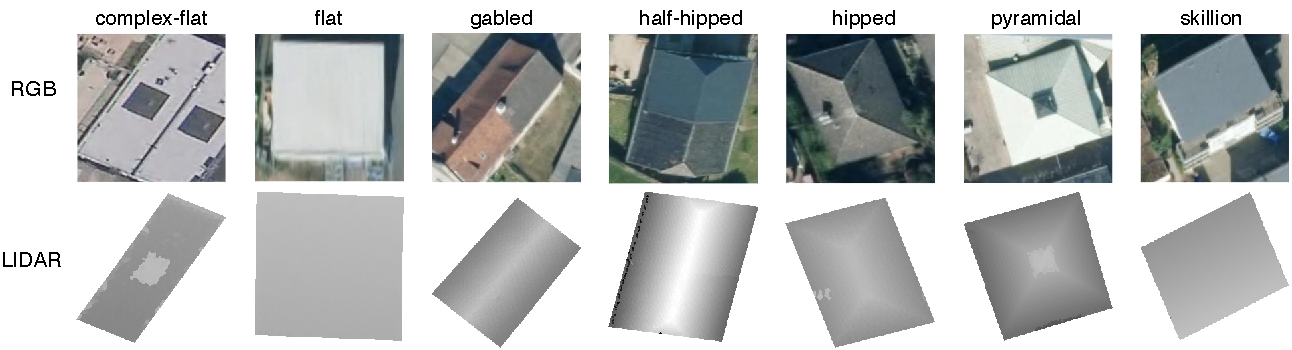
\includegraphics[width=0.99\textwidth]{chapter_4_roofshape/imgs/RoofShapes.pdf}
\caption{Satellite (RGB) and LiDAR example images of roof shapes.}
\label{fig:ch1_rooftop_shape_examples}
\end{figure}


\paragraph{Map based Planner}


% Urban areas typically do not offer classic emergency landing sites such as unpopulated open fields. This requires a planner to consider unconventional yet safe alternatives.

% We propose flat building rooftops as viable urgent landing sites for small UAS. During landing site selection, a map-based planner must be able to assess \emph{landing site risk} posed to the aircraft and bystanders at touchdown. The UAS may pose risk to people and property it overflies enroute, so the planner must also assess \emph{path risk} once the landing flight plan is known.  Landing site and path risk together offer an estimate of \emph{total risk}.

Map data used for urgent landing planning must have high integrity and low-latency access to support timely decision making. This dissertation proposes an offline data processing pipeline and online multi-objective, multi-goal landing planner that enable a UAS to minimize total risk when a nearby landing is required. Landing site and local area map information is pre-processed and stored onboard.  Roof shape classifiers and Polylidar3D are both used to identify flat-like rooftops and extract landing surfaces as polygons. Geometric algorithms are used to process flat rooftop polygons to find the largest inscribed circle that maximizes distance to obstacles and defines optimal touchdown location on each flat roof.  A multi-goal real-time landing planner explores available ground and rooftop landing sites likely to minimize overall total risk while greedily pruning options known to have higher risk.  Pareto fronts over landing site and path risk are generated for three urban regions: Witten, Germany; Ann Arbor, Michigan; and mid-town Manhattan in New York City. We statistically analyze results with respect to availability and quality of landing sites as well as execution time of the map-based planner.

\paragraph{Landing Site Identification and Selection Experiments (In Progress and Proposed)}

A small UAS should utilize available sensors to verify a safe touchdown point upon approach to a landing site. We build upon our previous methods for offline landing site identification and selection to  use on-board sensors generating point clouds in real-time. Prior work has investigated converting these point clouds to 2D disparity grids \cite{desaraju_vision-based_2015} or probabilistic elevation maps \cite{forster_continuous_2015}. These methods then apply computer vision kernels over the grids to smooth and identify ``flat'' touchdown points. 
% Sensors such as LiDAR, RGBD cameras, or monocular cameras utilizing Structure from Motion (SfM) can generate 3D point clouds of the landing site. 
An alternative to operating over a discretized image space is modelling the 3D mesh of the roof. Polylidar3D can be used to rapidly construct a surface mesh and extract polygonal representations of all flat surfaces while accounting for obstacles. Afterward the largest inscribed circle in each polygon is defined. For the final dissertation,  flight experiments with small multicopter UAS carrying LiDAR sensors will be conducted to demonstrate and evaluate real-time map generation for landing site safety validation (in areas with small UAS landing site maps) or real-time landing identification and selection (in areas without small UAS landing site maps). Tests will be conducted in the M-Air netted flight facility where motion capture can provide ground truth data to be compared with UAS-generated landing site maps and decisions. 


\paragraph{Contributions and Innovations \\}
% \vspace{1.5cm}
Specific contributions of this dissertation include: % things that have taken time / effort

\begin{itemize}[noitemsep]
  \item A faster open source library for non-convex (multi)polygon extraction from 2D point sets. An open source benchmark comparison of leading non-convex polygon extraction techniques in terms of accuracy and speed is provided. %\cite{Castagno_Github_Polylidar}.
%   \item An open source benchmark comparison of leading concave polygon extraction techniques from 2D point sets in terms of accuracy and speed.
  \item An efficient and versatile open source framework, Polylidar3D,  for non-convex (multi)polygon extraction from 3D data representing flat surfaces. Polylidar3D can handle unorganized and organized 3D point clouds as well as triangular meshes. Computation time is minimized with CPU multi-threading and GPU acceleration. %\cite{Castagno_Github_Polylidar}
  \item Multiple open source and reproducible experiments showing qualitative and quantitative benchmark results of Polylidar3D applied to sensors including LiDAR and RGBD cameras.
  \item A fast open source dominant plane normal estimation library, FastGA,  using a novel Gaussian Accumulator with efficient search.
  \item A deep learning framework for predicting roof shapes from a fusion of satellite image, airborne LiDAR point cloud, and existing building outline data. Over 4,500 buildings rooftops spanning three cities have been manually classified  for training, validation, and testing.
  \item A multi-goal planner that guarantees a risk-optimal solution is found rapidly by avoiding exploration of high-risk options. Plans are optimized over a combination of landing site and path risk metrics.
  \item (Proposed) Experimental UAS results of real-time landing site validation or identification/selection with Polylidar3D.
\end{itemize}
 
Specific innovations of this dissertation are: % things that have taken time / effort

\begin{itemize}[noitemsep]
      \item A novel computationally-efficient algorithm to extract non-convex polygons from 2D point sets while accounting for holes. The proposed method utilizes half-edge boundary following with edge-case detection instead of alternatives such as the expensive union of triangles.
      \item The first parallelized non-convex polygon extraction framework working with several forms of 3D data. Polygons represent dominant planar surfaces with interior holes representing the shape of obstacles embedded on their surface. Polylidar3D's speed and data input versatility allow its use for many applications.
    %   Triangle primitives are grouped according to dominant plane normals for which region growing occurs in parallel. Polygon extraction of segmented planar regions are spawned as dynamic tasks in a thread-pool. 
      \item The first large-scale multi-city analysis for predicting roof shapes. The provided annotated dataset contains diverse examples from small to large metropolitan city centers. 
      \item The first rigorous method to incorporate flat rooftops as candidate landing sites for urgent landing of small UAS in cities.  Optimal touchdown sites on rooftop surface are determined using geometric methods with risk evaluated according to size and proximity to alternative touchdown sites.
\end{itemize}


% Open Source C++ libraries (with Python bindings) are released at the following links:

% \begin{itemize}
%     \item Contribution 1 - {\small{ \url{https://github.com/JeremyBYU/polylidar/tree/polylidar2d}}}
%     \item Contribution 2 - {\small{ \url{https://github.com/JeremyBYU/polylidar}}}
%     \item Contribution 3 - {\small{\url{https://github.com/JeremyBYU/FastGaussianAccumulator}}}
%     \item Contribution 7 - TBD
% \end{itemize}

% Open Data sets are released at the following links:

% \begin{itemize}
%     \item Classified Roof Shape - {\small \url{https://www.mdpi.com/1424-8220/18/11/3960/s1}}
% \end{itemize}


\paragraph{Products}
Publications, software, and datasets connected to this dissertation are:
\vspace{0.2cm}

\textbf{Conference}
\vspace{0.20cm}
\begin{itemize}[noitemsep]
    \item J. Castagno, C. Ochoa, and E. Atkins, ``Comprehensive Risk-based Planning for Small Unmanned Aircraft System Rooftop Landing,” in 2018 \emph{International Conference on Unmanned Aircraft Systems} (ICUAS), Jun. 2018, pp. 1031–1040, doi: 10.1109/ICUAS.2018.8453483.
    \item K. McDonough, J. Castagno, and J. Player, ``RANGR: Risk Aware Navigation and Gudiance Resilience,” presented at the \emph{AUVSI Xponential}, Denver, CO, USA, May 2018.
	\item J. Castagno and E. M. Atkins, ``Automatic Classification of Roof Shapes for Multicopter Emergency Landing Site Selection,” in 2018 \emph{Aviation Technology, Integration, and Operations Conference, American Institute of Aeronautics and Astronautics}, 2018.
\end{itemize}

\vspace{0.25cm}

\textbf{Journal}

\vspace{0.20cm}
\begin{itemize}[noitemsep]
    \item J. Castagno, M. Romano, P. Kuevor, and E. Atkins, ``Multi-UAV Wildire Boundary Estimation using a Semantic Segmentation Neural Network,” \emph{Journal of Aerospace Information Systems}. Sumbitted under review.
    \item J. Castagno and E. Atkins, ``Map-Based Planning for Small Unmanned Aircraft Rooftop Landing (In Press),” in \emph{Handbook on Reinforcement Learning and Control}, Springer, 2021. In Press.
    \item J. Castagno and E. Atkins, “Polylidar3D - Fast Polygon Extraction from 3D Data,” \emph{Sensors}, vol. 20, no. 17, Art. no. 17, Jan. 2020, doi: 10.3390/s20174819.
    \item J. Castagno and E. Atkins, “Polylidar - Polygons From Triangular Meshes,” \emph{IEEE Robotics and Automation Letters}, vol. 5, no. 3, pp. 4634–4641, Jul. 2020, doi: 10.1109/LRA.2020.3002212.
    \item J. Castagno and E. Atkins, “Roof Shape Classification from LiDAR and Satellite Image Data Fusion Using Supervised Learning,” \emph{Sensors}, vol. 18, no. 11, Art. no. 11, Nov. 2018, doi: 10.3390/s18113960.
\end{itemize}

\textbf{Open Source C++ libraries (with Python bindings)}

\begin{itemize}[noitemsep]
    \item J. Castagno, ``Polylidar3D,''   [Online]  Available: \url{https://github.com/JeremyBYU/polylidar}, 2020.
    \item J. Castagno, ``Fast Gaussian Accumulator,''   [Online]  Available: \url{https://github.com/JeremyBYU/FastGaussianAccumulator}, 2020.
    \item J. Castagno, ``Organized Point Filters,''   [Online]  Available: \url{https://github.com/JeremyBYU/OrganizedPointFilters}, 2020.
\end{itemize}

\textbf{Open Data Sets}

\begin{itemize}[noitemsep]
    \item J. Castagno, ``Annotated Roof Shape Dataset,''   [Online]  Available: \url{https://www.mdpi.com/1424-8220/18/11/3960/s1}, 2018.
\end{itemize}
